\documentclass[a4paper]{article}
\usepackage[utf8]{inputenc}
\usepackage[T1]{fontenc}      
\usepackage[frenchb]{babel} %utilisation du package français
%
\usepackage{textcomp}% améliore certains symboles de bases
\usepackage{lmodern}% remplace la police ComputerModern par LatinModern (+ mieux bien)
%
\usepackage[a4paper]{geometry} % Pour avoir les marges pour du papier A4
%
\usepackage[intlimits, leqno]{amsmath}% ams-mathh ! avec numérotation des équations à gauche et intégrales avec limites dessous
\usepackage{mathtools}% compléments à amsmath
\usepackage{amssymb,amsfonts}% symboles mathématiques supplémentaires
\usepackage{bm}% symbole math gras
\usepackage{amsthm}% environnement ams-theorem
\usepackage{array}% ajoute des options aux environnements tabular et arrray, permet de centrer
\usepackage{mathrsfs}% permet d'utiliser matcal
\usepackage{theoremref} %permet de citer les thm

\usepackage{here}
%
\usepackage{todonotes} %ajouter des commentaires
%\usepackage[disable]{todonotes}%cache les commentaires
\usepackage{datetime} %ajoute la date et l'heure
\usepackage{here} % permet d'utilser H, h pour place les figures
%
%
%
\newtheorem{lem}{Lemme}[section]
%\newtheorem{AFaire}[lemma]{A faire}% peut enlever à la fin
%\newtheorem{Next}[lemma]{Possible continuation}% peut enlever à la fin
\newtheorem{conjecture}[lem]{Conjecture}
\newtheorem{cor}[lem]{Corolaire}
\newtheorem{prop}[lem]{Proposition}
\newtheorem{question}[lem]{Question}
\newtheorem{thm}[lem]{Théorème}
\theoremstyle{remark}% texte en roman
\newtheorem{claim}[lem]{Affirmation}
\newtheorem{defn}[lem]{Définition}
\newtheorem{exmp}[lem]{Exemple}
\newtheorem{fact}[lem]{Fait}
\newtheorem{notation}[lem]{Notation}
\newtheorem{rem}[lem]{Remarque}
\newtheorem{scholion}[lem]{Scholion}
\newtheorem{exo}{Exercice}
\newtheorem{quest}[lem]{Question}
%
%
%
\DeclareMathOperator\Aut{Aut} 
\DeclareMathOperator\Cay{Cay}
\DeclareMathOperator\cl{Cl}
\DeclareMathOperator\fix{Fix}
\DeclareMathOperator\GL{GL}		%groupe linéaire
\DeclareMathOperator\im{im}
\DeclareMathOperator\id{Id}
\DeclareMathOperator\orbite{O}
\DeclareMathOperator\ppcm{ppcm}
\DeclareMathOperator\pgcd{pgcd}
\DeclareMathOperator\Sch{Sch}
\DeclareMathOperator\sign{sign}
\DeclareMathOperator\SL{SL}		
\DeclareMathOperator\stab{Stab}
\DeclareMathOperator\supp{supp}
%
\DeclarePairedDelimiter\abs{\lvert}{\rvert}
\DeclarePairedDelimiter\gen{\langle}{\rangle}
\DeclarePairedDelimiter\set{\lbrace}{\rbrace}
\DeclarePairedDelimiter\parent{\lparen}{\rparen}
\DeclarePairedDelimiter\norm{\|}{\|}
%
\newcommand*{\actsGroup}{\curvearrowright}% sementic command for G acts X
\newcommand*{\iso}{\cong}% isomorphisme,commande sémantique (\simeq ou \cong)
\renewcommand*{\H}{\mathcal{H}}
\renewcommand*{\phi}{\varphi}
%
\newcommand*{\field}[1]{\mathbf{#1}}
\newcommand*{\N}{\field{N}}
\newcommand*{\Z}{\field{Z}}
\newcommand*{\Q}{\field{Q}}
\newcommand*{\R}{\field{R}}
\newcommand*{\C}{\field{C}}
%
\newcommand*{\B}{\mathcal{B}_1}
\renewcommand*{\H}{\mathcal{H}}
\renewcommand*{\S}{\mathcal{S}}
\newcommand*{\T}{\mathcal{T}}
%
%
%
\title{Action des produits en couronne sur des complexes cubiques CAT(0)}
\author{Grégoire Schneeberger}
\date{\today \quad \currenttime}
%
%
%
\begin{document}
\maketitle
\section{Introduction}
Comprendre les actions des groupes sur les arbres nous permet d'obtenir une bonne quantité d'informations sur ceux-ci (Basse-Serre). Si on cherche à généraliser cela, les complexes cubiques CAT(0) sont des espaces qui sont une généralisation naturel des arbres. Il y a des grandes familles de groupes qui agissent sur des complexe cubique CAT(0) et cela nous donne une grande quantité d'information sur ceux ci (Propriété (T), Propriété de Haagerup, alternative the Tits, etc). 
%
%
\section{Complexes cubiques CAT(0)}
\begin{defn}
Un complexe cubique est un recollement de cube par isométries. On peut le munir de la métrique induite par la métrique euclidienne des cubes. Il est dit $CAT(0)$ si il c'est un espace $CAT(0)$ pour cette métrique.
\end{defn}
%
 \begin{figure}[H]
 \centering
 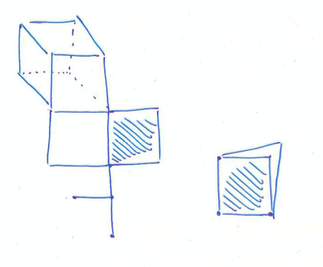
\includegraphics[scale=.5]{cc.png}.
\end{figure}
\begin{defn}
Soit $v$ un sommet d'un complexe cubique $X$. Le liens de $v$ est le complexe construit de la manière suivante : On met un sommet pour chaque arrêtes adjacente à $v$ puis deux sommets sont lié si les arètes correspondantes sont dans le bord du carré commun, etc. Un complexe simplicial est un drapeau, si chaque sous-graphe complet est le 1-squelette d'un simplexe, c-à-d qu'il n'y a pas de squelette de simplexe qui ne soit pas rempli. 
\end{defn}
%
\begin{thm}[Gromov '87, Leary '13]
Soit $X$ un complexe cubique simplement connexe (de dimension finie ou infinie). C'est un espace CAT(0) si et seulement si les liens de tout les sommets sont des drapeaux. 
\end{thm}
On va appeler de tels complexes de complexes cubique CAT(0). 
\begin{exmp}
\item Dans le cadre des graphes, simplement connexe = arbre
 \begin{figure}[H]
 \centering
 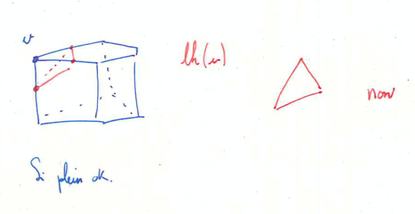
\includegraphics[scale=.5]{lk.png}.
\end{figure}
\end{exmp}
Une action d'une groupe $G$ sur un complexe cubique CAT(0) doit préserver la structure de complexe cubique.
%
\begin{defn}
On définit un hyperplan plan (combinatoire) comme une classe d'équivalence d'arrètes qui sont 2 à 2 des sommets opposés d'un carré. On peut aussi définir un hyperplan géométrique à partir des hyperplans combinatoires. 
\end{defn}
%
 \begin{figure}[H]
 \centering
 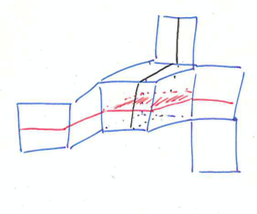
\includegraphics[scale=.5]{hyp.png}.
\end{figure}
%
\begin{thm}[Sageev '95]
Si $X$ est un complexe cubique CAT(0), alors chaque hyperplan coupe le complexe en 2 exactement composantes connexes.
\end{thm}
%
\begin{defn}
Un groupe $G$ agit \emph{essentiellement} sur un complexe cubique CAT(0) si sont action est transitive sur les hyperplans et si les orbites des sommets sont non bornées.
\end{defn}
%
%
\section{Bouts}
Notion de bout pour les groupes introduite par Hopf dans \cite{Hopf1944}
\begin{defn}
Soit $G$ un groupe de type fini et $S$ un système de générateur. On peut définir le graphe de Cayley de $G$ associé à $S$. Pour un sous-groupe $H<G$ on définit le graphe de Schreier $\Sch(G,H,S)$ comme le graphe dont les sommets sont les éléments de $G/H$ et deux sommets $gH$ et $g'H$ sont lié par une arrète si il existe $s \in S$ tel que $g'H = sgH$.
\end{defn}
%
\begin{defn}
Soit $X$ un graphe et $K \subset X$ un ensemble fini de sommet. $E(K)$ donne le nombre de composantes connexes infinies de $X \setminus K$. On définit le nombre de bout du graphe $X$ comme 
\begin{equation*}
e(X) = \sup \parent*{e(K) : K \subset X \text{ fini}}.
\end{equation*}
\end{defn}
%
\begin{defn}
Soit $G$ un groupe de type fini engendré par $S$ et $H<G$ un sous-groupe. On note $e(G)$ le nombre de bout de $\Cay(G,S)$ et $e(G,H)$ le nombre de bout de $\Sch(G,H,S)$.
\end{defn}
%
\begin{rem}
Le nombre de bout ne dépend pas du système de générateur, les notations $e(G)$ et $e(G,H)$ ne sont donc pas ambiguës.
\end{rem}
\begin{exmp}
\begin{enumerate}
\item Les groupes finis ont $0$ bouts
\item $\Z$ possède 2 bouts
\item $\Z^2$ possède 1 bouts
\item Groupe libre possède une infinité de bouts
\end{enumerate}
\end{exmp}
%
\begin{rem}
Le nombre de bout reste invariant par quotient par sous-groupe fini.
\end{rem}
%
\begin{quest}
Quels sont les nombres de bouts possibles pour un groupe ?
\end{quest}
%
Stallings \cite{Stallings1971} pour les groupes de types finis et Dicks-Dunwoody pour le cas général \cite{Dicks1989} car on peut définir ces notions pour des groupes qui ne sont pas de type fini, en considérant des compactes à la place des ensembles finis.
\begin{thm}[Stallings '71, Dicks-Dunwoody '89]
Soit $G$ un groupe de type fini Alors $e(G) \in \set*{0,1,2,\infty}$. De plus,
\begin{enumerate}
\item \label{type1} $e(G) = 0$ si et seulement si $G$ est fini.
\item \label{type2} $e(G) = 2$ si et seulement si $G$ est virtuellement $\Z$.
\item\label{type3} $e(G) = \infty$ si et seulement si un des cas suivants est vérifié :
	\begin{enumerate}
	\item $G \iso B *_C D$ avec $C$ fini et $B \neq C \neq D$ et $G$ pas de type \ref{type2}
	\item $G \iso B *_C x$ avec $C$ fini $G$ pas de type \ref{type2}
%	\item $G$ est infini-dénombrable et localement fini. \todo{verifier} 
	\end{enumerate}
\end{enumerate}
\end{thm}
%
%
\begin{cor}
Les groupes des torsions infinis ont 1 bouts
\end{cor}
%
\begin{proof}
Par le théorème précédent, si $e(G)>1$ alors $G$ est soit virtuellement cyclique, dans ce cas il y a un élément d'ordre infini, soit une produit amalgamé et dans ce cas l'élément $bd$ ou $bx$ est aussi d'ordre infini.
\end{proof}
%
%
Le nombre de bouts pour graphe de Schreier a été étudié par \cite{Scott1977,Swarup1977,Muller1981,Kropholler1989}. On peut trouver des graphes de Schreier avec un nombre arbitraire de bouts en utilisant le résultat de Leemann qui dit que chaque graphe régulier de degré pair peut être vu comme un Schreier (modulo une petite condition sur les boucle).
%
%
Sageev a démontré une manière de prouver qu'un groupe possède un graphe de Schreier avec au moins 2 bouts inspirée de la théorie de Basse-Serre (produit amalgamé si action sans point fixe sur un arbre)
%
\begin{defn}
On définit par $\B$ la classe des groupes qui possède uniquement des graphes de Schreier à 0 ou 1 bouts, c-à-d
\begin{equation*}
\B \coloneqq \{G : G \text{ est un groupe et } \forall H \leq G, e(G,H) \leq 1\}.
\end{equation*}
\end{defn}
%
%

Il y a un lien entre le nombre de bout et les actions sur les complexes cubiques CAT(0).
%
\begin{thm}[Sageev '95]
Un groupe $G$ de type fini n'est pas dans $\B$ si et seulement si il admet un action essentielle sur un complexe cubique CAT(0)
\end{thm}
%
\begin{proof}
Si on se donne le graphe de Schreier, on construit explicitement le complexe et l'action. Dans l'autre sens, on prend la stabilisateur d'un hyperplan. 
\end{proof}
%
%
\section{Propriété (T)}
Introduite en 1967 par Kazhdan dans \cite{Kazhdan1967}. Source principal : \cite{Bekka2008}
\begin{defn}
Soit $G$ un groupe topologique et $\set*{\pi, \H}$ un représentation unitaire de celui-ci. Un vecteur $\xi \in \H$ est dit $(Q,\epsilon)$-invariant, pour $\epsilon$ un réel et $Q \subset G$, si on a $\norm{q \xi - \xi} < \epsilon \norm{\xi}$ pour tout $q \in Q$. Un groupe $G$ possède la propriété (T) de Kazhdan si il existe $\epsilon>0$ et un compact $Q$ tel que si possède un vecteur qui est $(Q,\epsilon)$-invariant alors il possède un vecteur non nul qui est $G$-invariant.
\end{defn}
%
Peut être vu comme une sorte d'opposé de moyennable. En effet
\begin{thm}
Un groupe $G$ localement compact possède la propriété (T) et est moyennable si et seulement si il est compact. 
\end{thm}
%
%
Exemples
\begin{enumerate}
\item Groupes compacts ont (T) (exercice) 
\item $\SL_n(\R)$ pour $n \geq 3$ a (T).
\item $\Z,\R$ pas (T)
\item $\SL_2(\Z)$ et $\SL_2(\R)$ ne possède pas (T).
\end{enumerate}
%
application : 
\begin{itemize}
\item  Construction de familles d'expanseurs
\item 
\end{itemize}
%
%
\section{Thm Niblo-Roller}
Niblo-Reeves '97 dans le cadre dimension finie.
\begin{thm}[Niblo-Roller '98]
Si un groupe n'est pas dans $\B$ alors il ne possède pas la propriété (T) de Kazhdan ou en d'autres mots, tout les groupes avec la propriété (T) sont dans $\B$
\end{thm}
\begin{proof}
Idée de la preuve. On utilise le thm 
\begin{thm}[Delorme-Guichardet]
Un groupe $G$ de type fini possède la propriété (T) si et seulement si chaque action de $G$ sur un espace de Hilert par isométries affines possède un point fixe. 
\end{thm}
Si $G$ n'est pas dans $\B$ alors il agit sans point fixe sur un CCC que l'on peut plonger dans un Hilbert. On peut prouver que l'on a donc une action sans point fixe sur un Hilbert ce qui est une condition suffisante à la perte de la propriété (T).
\end{proof}
%
%
Exemple d'application :
Les groupes de Burnside libre $B(m,n)=\gen{s_1,\ldots,s_m \mid w(s_1,\ldots,s_m)^n=1}$ avec $w(s_1,\ldots,s_m)$ tout les mots de l'alphabet $\{s_1,\ldots,s_m\}$.
%
%
\begin{thm}[Osajda '18]
Si le groupe de Burnside libre $B(m,n)$ est infini alors pour $k>1$, le groupe $B(m,kn)$ agit sur un complexe cubique CAT(0) sans point fixe et par conséquent ne possède pas la propriété (T).
\end{thm}
%
\begin{proof}
Il y a deux possibilités : 

On construit un CCC avec une action essentielle (preuve originale). Dans le papier, pas la même construction quand Sageev, car il n'exhibe pas de graphe de Schreier à au moins 2 bouts.
\end{proof}
\begin{quest} \label{quest}
Existe-t-il des groupes sans la propriété (T) qui sont dans $\B$.
\end{quest}
%
On peut répondre à ce genre de question dans le cadre d'espaces plus généraux comme celui des espaces à murs mesurés.
Un candidat serait les monstres de Tarski.
\begin{defn}
Un groupe $G$ est un monstre de Tarski si il est infini et si il existe un premier $p$ tel que chaque sous-groupe non trivial est isomorphe à $C_p$.
\end{defn}
%
La première construction des monstre de Tarski est due à Olshaskii en 1979. Il a montré que pour tout premier $p>10^{75}$ il y a une infinités non-dénombrable de monstre de Tarski non-isomorphes. Le meilleur résultat actuel est \cite{Adyan1991} qui montre que pour tout $n>1003$ impaire, il existe des groupes infinis, de rang 2, tel que chaque sous-groupes est inclus dans un sous-groupe $C_n$.
Les monstres de Tarski sont tous dans $\B$. 
%
\begin{proof}
Les monstres de Tarski sont de torsion donc leur graphes de Cayley a 1 bouts. De plus tout les sous-groupes sont finis, donc tout les Schreier ont aussi 1 bouts.
\end{proof}
%
Par contre on ne sait pas si ils ont la propriété (T). 
\begin{quest}
Est ce que les groupes $\T_p$ possède la propriété (T). 
\end{quest}
%
%
\section{Produits en couronnes}
On peut prouver Osajda avec les produits en couronnes%
\begin{defn}
Soient $G,H$ deux groupes et $X$ un ensemble sur lequel agit $H$. Il y a donc une action de $H$ sur $\bigoplus_X G$ via en effet pour $\phi \in \bigoplus_X G$ et $h \in H$ on défini $h \cdot \phi (x) = \phi (h^{-1} \cdot x)$. On définit les produits en couronne $G \wr_X H = \bigoplus_X G \rtimes H$ avec l'opération 
\begin{equation*}
(\phi_1,h_1)(\phi_2,h_2) = (\phi_1 (h_1^{-1} \cdot \phi_2), h_1h_2).
\end{equation*}
Avec $(h\cdot \phi)(x)=\phi(h^{-1}\cdot x)$. On note $G \wr H$ pour $\bigoplus_H G \rtimes H$.
\end{defn}
%
Une autre preuve de Osajda 
\begin{proof}[Une seconde preuve de Osajda]
On considère le produit en couronne $W=\Z/k\Z \wr B(m,n)$. L'ordre de chaque élément divise $kn$. C'est donc un quotient de $B(m+1,kn)$. On applique le résultat suivant 
%
\begin{thm}[Cherix-Martin-Valette '04, Neuhauser '05]
Soit $G,H$ deux groupes de types fini et $X$ un $H$-ensemble. Alors $G \wr_X H$ à la propriété (T) si et seulement si $G,H$ l'ont et si $X$ est fini.\end{thm}
Le groupe $W$ n'a pas (T) si $k >1$ et si $B(m,n)$ est infini
\end{proof}
Un bon candidat pour répondre à la question~\ref{quest} serait le groupe $\Gamma = \Z/2\Z \wr M$ avec $M$ un monstre de Tarski. En effet ce groupe n'a pas la propriété (T) et les sous-groupes de $M$ sont fini

On peut se demander si de tels produit en couronne sont dans $\B$ ou non.
%
\begin{thm}[Leemann-S.]
Soient $G,H$ deux groupes de types finis et $X$ un ensemble sur lequel $H$ agit transitivement. Le produit en couronne $G \wr_X H = \bigoplus_X G \rtimes H$ n'est pas dans $\B$ si une des trois conditions suivantes est satisfaite :
\begin{enumerate}
\item $G$ n'est pas dans $\B$.
\item $H$ n'est pas dans $\B$.
\item $X$ est infini.
\end{enumerate}
\end{thm}
%
\begin{cor}
Soient $G,H$ deux groupes de types finis et $X$ un ensemble sur lequel $H$ agit transitivement. Si il existe une action essentielle de $G$ ou $H$ sur un complexe cubique CAT(0) ou si $X$ est infini, alors il existe une action essentielle du produit en couronne $G\wr_XH$ sur un complexe cubique CAT(0).
\end{cor}
%
\begin{proof}
On utilise Sageev
\end{proof}
%
\begin{proof}[Démonstration du Théorème]
Commençons par de la notation. On note $\Gamma = G \wr_X H$, les systèmes de générateurs $G=\gen{S}, H=\gen{S'}$ et on choisi un point $x_0$ arbitrairement dans $X$. Le groupe $\Gamma$ est engendré par l'ensemble suivant 
\begin{equation*}
\S=\set*{\left(\delta_{x_0}^s,e_H\right) : s \in S} \cup \set*{(0,s') : s' \in S'} 
\end{equation*}
où $\delta_{x_0}^s (y) = 
\begin{cases}
e_G &y \neq x_0 \\
s	&y=x_0
\end{cases}$.
Traitons maintenant les trois cas séparément.

Supposons que $X$ soit infini. On peut définir un action de $\Gamma$ sur $\Omega = G \times X$ de la manière suivante. Soit $(\phi,h) \in \Gamma$ et $(g,x) \in \Omega$,
%
\begin{equation*}
(\phi,h) \cdot (g,x) =(\phi(hx)g,hx).
\end{equation*}
%
C'est bien une action de groupe : 
%
\begin{align*}
\left( (\phi_1,h_1)(\phi_2,h_2)\right) \cdot (g,x) 	&= (\phi_1*h_1\phi_2,h_1h_2) \cdot (g,x) \\
												&= ((\phi_1*h_1\phi_2)(h_1h_2x) g, h_1h_2x) \\
												&= (\phi_1(h_1h_2x)  \phi_2(h_2h)  g, h_1h_2x) \\
												&=  (\phi_1,h_1)\cdot((\phi_2,h_2)\cdot(g,x)).
\end{align*}
%
De plus elle est transitive, car pour tout élément $(g_1,x_1),(g_2,x_2)$ de $\Omega$, il existe $h_1$ tel que $h_1x_1=x_2$ et une fonction $\phi$ telle que  $\phi(h_1x_1)=g_2g_1^{-1}$, ce qui nous donne
% 
\begin{equation*}
(\phi,h_1)\cdot(g_1,x_1)=(g_2,x_2)
\end{equation*}
%
L'ensemble $\Omega$ peut donc être vu comme le graphe $\Sch\parent*{\Gamma, \stab\parent*{e_G,x_0},\S}$. On peut découper ce graphes en feuilles de la forme $\set*{g} \times X$, notées $\Omega_g$. Si on regarde les arrêtes étiquetées par $\set*{(0,s') : s' \in S'}$, on remarque que les sommets de $\Omega_g$ sont en bijection avec $X$, car l'action est transitive et que l'on retrouve le graphe de l'action de $H$ sur $X$. Maintenant regardons les arrêtes de la forme $\set*{\parent*{\delta_{x_0}^s,e_H} : s \in S}$. Si on calcule,
\begin{align*}
\parent*{\delta_{x_0}^s,e_H}\parent*{g,y} 	&= \parent*{\delta_{x_0}^s(e_H y)g,e_Hy}	\\
											&= 
\begin{cases}
\parent*{g,y}	& y \neq x_0	\\
\parent*{sg,y}	& y = x_0
\end{cases}.
\end{align*}
Ces arrêts forment des boucles sur tout les sommets de $\Omega_g$ excepté en $(g,x_0)$. Si on enlève ce somment, on déconnecte cette feuille qui est infinie et on a donc au moins deux bouts. On voit qu'en réalité, ce graphe de Schreier possède un nombre de bouts égal au cardinal de $G$.

Maintenant supposons que $G$ n'est pas dans $\B$. Il existe donc un sous-groupe $K \leq G$ tel que $e(G,H) \geq 2$. On va construire le même genre d'action que ci-dessus, mais maintenant sur $G/K \times X$, via 
\begin{equation*}
(\phi,h) \cdot (gK,x) =(\phi(hx)gK,hx).
\end{equation*}.
De la même manière, on vérifie que c'est bien une action
\begin{align*}
\left( (\phi_1,h_1)(\phi_2,h_2)\right) \cdot (gK,x) 	&= (\phi_1+h_1\phi_2,h_1h_2) \cdot (gK,x) \\
												&= ((\phi_1+h_1\phi_2)(h_1h_2x) gK, h_1h_2x) \\
												&= (\phi_1(h_1h_2x)  \phi_2(h_2h)  gK, h_1h_2x) \\
												&=  (\phi_1,h_1)\cdot((\phi_2,h_2)\cdot(gK,x)).
\end{align*}
et qu'elle est transitive
%
\begin{equation*}
(\phi,h_1)\cdot(g_1K,x_1)=(g_2K,x_2)
\end{equation*}
si $h_1x_1=x_2$ et $\phi(h_1x_1)=g_2g_1^{-1}$. On peut découper notre graphe de Schreier en feuille de la même manière. La structure des arrêtes est la même elle aussi. C'est-a-dire que Chaque feuille est une copie du graphe de l'action de $H$ sur $X$ et que les arrêtes de la forme $ \set*{\left(\delta_{x_0}^s,e_H\right)}$ forment des boucles sur tout les sommets exceptés ceux de la forme $(-,x_0)$. Si on se restreint aux sommets de cette forme et à ces arrêtes, on obtient le graphe de Schreier $\Sch(G/K,S)$, qui possèdes au moins 2 bouts. On peut donc enlever un nombre fini de sommet et déconnecter notre graphe. 

Supposons que $H$ n'est pas dans $\B$. Il y a donc un sous-groupe $K \leq H$ tel que $e(H,K) \geq 2$ Dans ce cas on regarde l'action de $\Gamma$ sur $H/K$ définie comme 
\begin{equation*}
(\phi,h)h'K=hh'K.
\end{equation*}
C'est bien une action et elle est transitive. Toutes les arrêtes de la forme $\left(\delta_{x_0}^s,e_H\right)$ forment des boucles alors que les autres sont exactement les arrêts de $\Sch(H/K,S')$ qui possède au moins 2 bouts. On peut, par conséquent, déconnecter ce graphe lui aussi.
\end{proof}
%
%
\nocite{*}
\bibliography{Neuchatel.bib}
\bibliographystyle{alpha}


\enddocument